
\section{图}
\label{sec:graphs}

\subsection{染色}
\begin{example}
  有一种四个人玩的牌,两人为一组。为了公平起见,规定同一方的两人必须都曾经合作过,或者都不曾合作过。那么只要有5个人,就一定能凑齐4个人按这种约定在一起打牌。
\end{example}
\begin{proof}[提示]对图形染色的策略特别适合用于解决此类问题。此处为印刷后方便辩认,不用染色,而是用实线与虚线表示不同的染色。
  
  5个点代表5个人,两人合作过则连实线,未合作过则连虚线。则总共有$C_5^2=10$条边。
  \begin{center}
    \begin{tikzpicture}[scale=.5]
      \begin{scope}
        \foreach \i in {1,2,3,4,5}{%
          \coordinate(N\i) at (360/5*\i:2);
          \node at (360/5*\i:3) {$N_\i$};
        }
        \tkzDrawPoints(N1, N2, N3, N4, N5);
        \node at (0,-4) {(a)};
      \end{scope}
      \begin{scope}[shift={(9,0)}]
        \foreach \i in {1,2,3,4,5}{%
          \coordinate(N\i) at (360/5*\i:2);
          \node at (360/5*\i:3) {$N_\i$};
        }
        \tkzDrawPoints(N1, N2, N3, N4, N5);
        \draw(N1)--(N2) (N3)--(N4);
        \node at (0,-4) {(b)};
      \end{scope}
      \begin{scope}[shift={(18,0)}]
        \foreach \i in {1,2,3,4,5}{%
          \coordinate(N\i) at (360/5*\i:2);
          \node at (360/5*\i:3) {$N_\i$};
        }
        \tkzDrawPoints(N1, N2, N3, N4, N5);
        \draw(N1)--(N2);
        \draw[dashed](N3)--(N4)--(N5)--cycle;
        \node at (0,-4) {(c)};
      \end{scope}
      \begin{scope}[shift={(0,-9)}]
        \foreach \i in {1,2,3,4,5}{%
          \coordinate(N\i) at (360/5*\i:2);
          \node at (360/5*\i:3) {$N_\i$};
        }
        \tkzDrawPoints(N1, N2, N3, N4, N5);
        \draw(N1)--(N2);
        \draw[dashed](N3)--(N4)--(N5)--cycle--(N1);
        \node at (0,-4) {(d)};
      \end{scope}
      \begin{scope}[shift={(9,-9)}]
        \foreach \i in {1,2,3,4,5}{%
          \coordinate(N\i) at (360/5*\i:2);
          \node at (360/5*\i:3) {$N_\i$};
        }
        \tkzDrawPoints(N1, N2, N3, N4, N5);
        \draw(N1)--(N2)--(N3)--cycle (N4)--(N1)--(N5)--(N2)--(N4) ;
        \draw[dashed](N3)--(N4)--(N5)--cycle;
        \node at (0,-4) {(e)};
      \end{scope}
    \end{tikzpicture}
  \end{center}
  原问题等价于在这样的图里总能找到两条同为实线或同为虚线的不共点的边。取定一条,不妨记为$N_1N_2$,且不妨假设此边为实线。考虑剩余三个点$N_3, N_4, N_5$,有两种情况:

  若该三点组成的三角形中有一条实线边,不妨假设为$N_3N_4$,如图(b),则连同$N_1N_2$,已经找到了两条不同顶点的实线边。

  若该三点组成的三角形全是虚线边,如图(c)。考虑剩余的边,若有一条是虚线,假设为$N_1N_3$,如图(d),则已经找到了两条不同顶点的虚线边。否则若剩余的边全是实线边,如图(e),则也容易找到两条不共点的实线边,比如$N_1N_5$和$N_2N_4$。
\end{proof}

\subsection{正则图}
\label{sec:regular-graph}

\begin{example}
  屋子里有若干个人,任意两个人都有恰好$1$个共同的朋友。这有可能吗?
\end{example}
\begin{proof}[提示]
  有可能。以$9$人为例,是朋友则连线,容易验证下图的$9$人关系中任意两人都恰好有一个共同的朋友。

  \begin{center}
  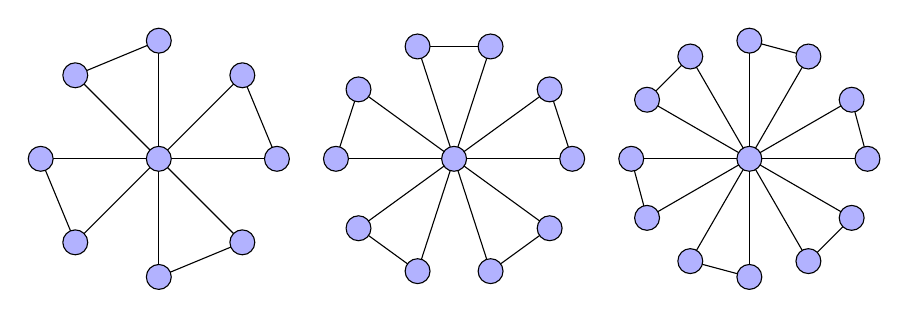
\begin{tikzpicture}[scale=1.5]
    \begin{scope}[shift={(0,0)}]
      \coordinate(A0) at (0,0);
      \coordinate(A1) at (0:1);
      \coordinate(A2) at (45:1);
      \coordinate(A3) at (90:1);
      \coordinate(A4) at (135:1);
      \coordinate(A5) at (180:1);
      \coordinate(A6) at (225:1);
      \coordinate(A7) at (270:1);
      \coordinate(A8) at (315:1);
      \foreach \p in {A1,A2,A3,A4,A5,A6,A7,A8}{
        \draw(A0)--(\p);
      }
      \foreach \x/\y in{A1/A2,A3/A4,A5/A6,A7/A8}{
        \draw(\x)--(\y);
      }
      \foreach \p in {A0,A1,A2,A3,A4,A5,A6,A7,A8}{
        \draw[fill=blue!30] (\p) circle(3pt);
      }
    \end{scope}
    \begin{scope}[shift={(2.5,0)}]
      \coordinate(A0) at (0,0);
      \coordinate(A1) at (0:1);
      \coordinate(A2) at (1*36:1);
      \coordinate(A3) at (2*36:1);
      \coordinate(A4) at (3*36:1);
      \coordinate(A5) at (4*36:1);
      \coordinate(A6) at (5*36:1);
      \coordinate(A7) at (6*36:1);
      \coordinate(A8) at (7*36:1);
      \coordinate(A9) at (8*36:1);
      \coordinate(A10) at(9*36:1);
      \foreach \p in {A1,A2,A3,A4,A5,A6,A7,A8,A9,A10}{
        \draw(A0)--(\p);
      }
      \foreach \x/\y in{A1/A2,A3/A4,A5/A6,A7/A8,A9/A10}{
        \draw(\x)--(\y);
      }
      \foreach \p in {A0,A1,A2,A3,A4,A5,A6,A7,A8,A9,A10}{
        \draw[fill=blue!30] (\p) circle(3pt);
      }
    \end{scope}
    \begin{scope}[shift={(5,0)}]
      \coordinate(A0) at (0,0);
      \coordinate(A1) at (0:1);
      \coordinate(A2) at (1*30:1);
      \coordinate(A3) at (2*30:1);
      \coordinate(A4) at (3*30:1);
      \coordinate(A5) at (4*30:1);
      \coordinate(A6) at (5*30:1);
      \coordinate(A7) at (6*30:1);
      \coordinate(A8) at (7*30:1);
      \coordinate(A9) at (8*30:1);
      \coordinate(A10)at (9*30:1);
      \coordinate(A11)at(10*30:1);
      \coordinate(A12)at(11*30:1);
      \foreach \p in {A1,A2,A3,A4,A5,A6,A7,A8,A9,A10,A11,A12}{
        \draw(A0)--(\p);
      }
      \foreach \x/\y in{A1/A2,A3/A4,A5/A6,A7/A8,A9/A10,A11/A12}{
        \draw(\x)--(\y);
      }
      \foreach \p in {A0,A1,A2,A3,A4,A5,A6,A7,A8,A9,A10,A11,A12}{
        \draw[fill=blue!30] (\p) circle(3pt);
      }
    \end{scope}
  \end{tikzpicture}
  \end{center}
  事实上,以上结论容易推广到任意大于$1$的奇数上。
\end{proof}

\begin{example}
  屋子里有若干个人,任意两个人都有恰好$2$个共同的朋友。这有可能吗?
\end{example}
\begin{proof}[提示]\mbox{}\par
  \begin{center}
  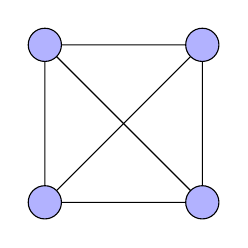
\begin{tikzpicture}[scale=2]
    \begin{scope}[shift={(0,0)}]
      \coordinate(A0) at (0,0);
      \coordinate(A1) at (1,0);
      \coordinate(A2) at (1,1);
      \coordinate(A3) at (0,1);
      \draw(A0)--(A1)--(A2)--(A3)--(A0)--(A2);
      \draw(A1)--(A3);
      \foreach \p in {A0,A1,A2,A3}{
        \draw[fill=blue!30](\p) circle(3pt);
      }
    \end{scope}  
  \end{tikzpicture}
  \end{center}
  如上图,有可能。  
\end{proof}

\begin{definition}[正则图,Regular Graph]
  若一个图的每个顶点都引出了相同数目的线,则称该为正则图。

  如果一个正则图有$v$个点,每个点都引出了$k$条线,并且它额外地满足,任意两个相邻的点之间都恰好有$\lambda$个公共邻点,任意两个不相邻的点之间都恰好有$\mu$个公共邻点,我们就说这个图是一个强正则图(Strongly Regular Graph),用符号$\mathrm{srg}(v,k,\lambda,\mu)$表示。
\end{definition}

\begin{example}[Shrikhande Graph]\mbox{}\par
  \begin{center}
    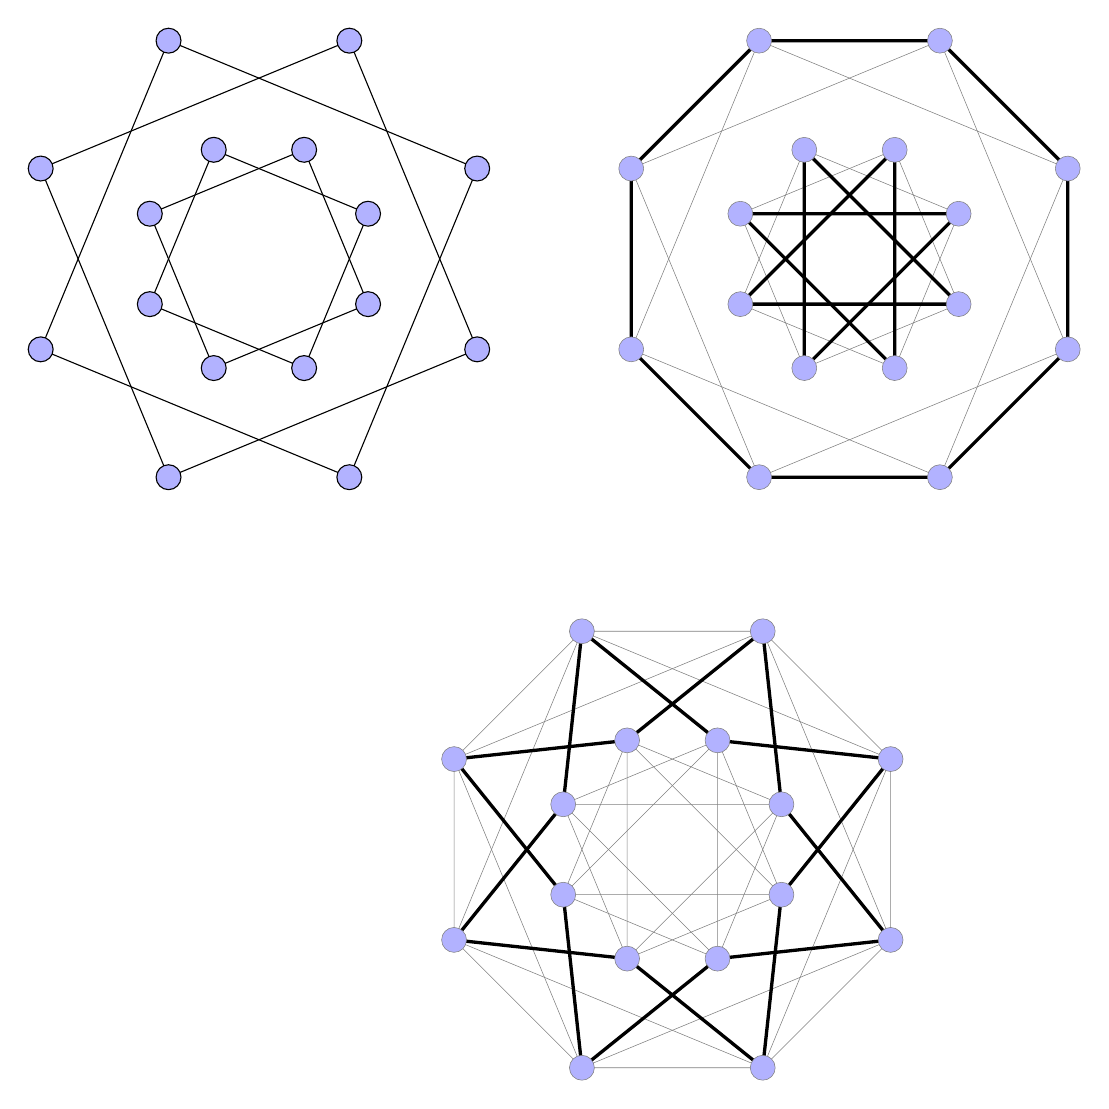
\begin{tikzpicture}[scale=1.5]
      \begin{scope}[shift={(0,0)}]
        \coordinate(A0) at ({(22.5 + 90 * 0)}:1);
        \coordinate(A1) at ({(22.5 + 90 * 1)}:1);
        \coordinate(A2) at ({(22.5 + 90 * 2)}:1);
        \coordinate(A3) at ({(22.5 + 90 * 3)}:1);
        \coordinate(B0) at ({(-22.5 + 90 * 0)}:1);
        \coordinate(B1) at ({(-22.5 + 90 * 1)}:1);
        \coordinate(B2) at ({(-22.5 + 90 * 2)}:1);
        \coordinate(B3) at ({(-22.5 + 90 * 3)}:1);

        \coordinate(C0) at ({(22.5 + 90 * 0)}:2);
        \coordinate(C1) at ({(22.5 + 90 * 1)}:2);
        \coordinate(C2) at ({(22.5 + 90 * 2)}:2);
        \coordinate(C3) at ({(22.5 + 90 * 3)}:2);
        \coordinate(D0) at ({(-22.5 + 90 * 0)}:2);
        \coordinate(D1) at ({(-22.5 + 90 * 1)}:2);
        \coordinate(D2) at ({(-22.5 + 90 * 2)}:2);
        \coordinate(D3) at ({(-22.5 + 90 * 3)}:2);
        
        \draw (A0)--(A1)--(A2)--(A3)--(A0);
        \draw (B0)--(B1)--(B2)--(B3)--(B0);
        \draw (C0)--(C1)--(C2)--(C3)--(C0);
        \draw (D0)--(D1)--(D2)--(D3)--(D0);
        \foreach \p in {A0,A1,A2,A3,B0,B1,B2,B3,C0,C1,C2,C3,D0,D1,D2,D3}{
          \draw[fill=blue!30](\p)circle(3pt);
        }
      \end{scope}
      \begin{scope}[shift={(2.5,0)}]
        \node at (0,0){\huge $\implies$};
      \end{scope}
      \begin{scope}[shift={(5,0)},help lines]
        \coordinate(A0) at ({(22.5 + 90 * 0)}:1);
        \coordinate(A1) at ({(22.5 + 90 * 1)}:1);
        \coordinate(A2) at ({(22.5 + 90 * 2)}:1);
        \coordinate(A3) at ({(22.5 + 90 * 3)}:1);
        \coordinate(B0) at ({(-22.5 + 90 * 0)}:1);
        \coordinate(B1) at ({(-22.5 + 90 * 1)}:1);
        \coordinate(B2) at ({(-22.5 + 90 * 2)}:1);
        \coordinate(B3) at ({(-22.5 + 90 * 3)}:1);

        \coordinate(C0) at ({(22.5 + 90 * 0)}:2);
        \coordinate(C1) at ({(22.5 + 90 * 1)}:2);
        \coordinate(C2) at ({(22.5 + 90 * 2)}:2);
        \coordinate(C3) at ({(22.5 + 90 * 3)}:2);
        \coordinate(D0) at ({(-22.5 + 90 * 0)}:2);
        \coordinate(D1) at ({(-22.5 + 90 * 1)}:2);
        \coordinate(D2) at ({(-22.5 + 90 * 2)}:2);
        \coordinate(D3) at ({(-22.5 + 90 * 3)}:2);
        
        \draw (A0)--(A1)--(A2)--(A3)--(A0);
        \draw (B0)--(B1)--(B2)--(B3)--(B0);
        \draw (C0)--(C1)--(C2)--(C3)--(C0);
        \draw (D0)--(D1)--(D2)--(D3)--(D0);

        \draw[very thick,color=black](D0)--(C0)--(D1)--(C1)--(D2)--(C2)--(D3)--(C3)--(D0);
        \draw[very thick,color=black](B3)--(A0)--(B2);
        \draw[very thick,color=black](B0)--(A1)--(B3);
        \draw[very thick,color=black](B1)--(A2)--(B0);
        \draw[very thick,color=black](B2)--(A3)--(B1);
        
        \foreach \p in {A0,A1,A2,A3,B0,B1,B2,B3,C0,C1,C2,C3,D0,D1,D2,D3}{
          \draw[fill=blue!30](\p)circle(3pt);
        }
      \end{scope}
      \begin{scope}[shift={(0,-5)}]
        \node at (0,0){\huge $\implies$};
      \end{scope}
      \begin{scope}[shift={(3.5,-5)},help lines]
        \coordinate(A0) at ({(22.5 + 90 * 0)}:1);
        \coordinate(A1) at ({(22.5 + 90 * 1)}:1);
        \coordinate(A2) at ({(22.5 + 90 * 2)}:1);
        \coordinate(A3) at ({(22.5 + 90 * 3)}:1);
        \coordinate(B0) at ({(-22.5 + 90 * 0)}:1);
        \coordinate(B1) at ({(-22.5 + 90 * 1)}:1);
        \coordinate(B2) at ({(-22.5 + 90 * 2)}:1);
        \coordinate(B3) at ({(-22.5 + 90 * 3)}:1);

        \coordinate(C0) at ({(22.5 + 90 * 0)}:2);
        \coordinate(C1) at ({(22.5 + 90 * 1)}:2);
        \coordinate(C2) at ({(22.5 + 90 * 2)}:2);
        \coordinate(C3) at ({(22.5 + 90 * 3)}:2);
        \coordinate(D0) at ({(-22.5 + 90 * 0)}:2);
        \coordinate(D1) at ({(-22.5 + 90 * 1)}:2);
        \coordinate(D2) at ({(-22.5 + 90 * 2)}:2);
        \coordinate(D3) at ({(-22.5 + 90 * 3)}:2);
        
        \draw (A0)--(A1)--(A2)--(A3)--(A0);
        \draw (B0)--(B1)--(B2)--(B3)--(B0);
        \draw (C0)--(C1)--(C2)--(C3)--(C0);
        \draw (D0)--(D1)--(D2)--(D3)--(D0);

        \draw(D0)--(C0)--(D1)--(C1)--(D2)--(C2)--(D3)--(C3)--(D0);
        \draw(B3)--(A0)--(B2);
        \draw(B0)--(A1)--(B3);
        \draw(B1)--(A2)--(B0);
        \draw(B2)--(A3)--(B1);

        \draw[very thick,color=black](B0)--(C0)--(B1);
        \draw[very thick,color=black](B1)--(C1)--(B2);
        \draw[very thick,color=black](B2)--(C2)--(B3);
        \draw[very thick,color=black](B3)--(C3)--(B0);

        \draw[very thick,color=black](A0)--(D1)--(A1);
        \draw[very thick,color=black](A1)--(D2)--(A2);
        \draw[very thick,color=black](A2)--(D3)--(A3);
        \draw[very thick,color=black](A3)--(D0)--(A0);
        
        \foreach \p in {A0,A1,A2,A3,B0,B1,B2,B3,C0,C1,C2,C3,D0,D1,D2,D3}{
          \draw[fill=blue!30](\p)circle(3pt);
        }
      \end{scope}
    \end{tikzpicture}
  \end{center}
  上面的第$3$个图就是Shrikhande Graph,它有$16$个顶点,$48$条连线,每个顶点恰好引出了$6$条连线。这是一个强正则图。
\end{example}